\chapter{Test and Evaluation}
\label{ch:evaluation}
%Aufbau der Messumgebung (1­2 Seiten)
%●
%Server/Betriebssystem etc.
%Datensätze
%Anfragen
%Systeme/Ansätze gegen die Sie sich vergleichen
%Wie messen Sie? Methodik und Maßeinheiten?
%Ist die Messung signifikant?
%Hypothesen/ Was erwarten Sie?
%
%Ergebnisse und Beobachtungen (3 ­4 Seiten)
%●
%Beschreibung  der Ergebnisse
%Diagramme
%Darstellen von Zusammenhängen
%Diskussion und Bewertung (3 ­4 Seiten)
%●
%Wurden Sie überrascht?
%Stimmten Ihre Hypothesen?
%Sind Sie besser, anders als das andere System?
%Wichtigster Erkenntnisgewinn 1
%Wichtigster Erkenntnisgewinn 2
%... .
%Wichtigster Erkenntnisgewinn N
%Anwendbarkeit? Szenario?
%Zusammenfassung (ca. 0,5 Seiten)
%●
%Was haben wir in diesem Kapitel gelernt?
%Wie passt das zur Zielstellung der Arbeit
%Wie passt das zum nächsten Kapitel?
%
%In this section, we will focus on testing and evaluating implemented profiling solution. Testing
%is necessary and extremely important phase in software development lifecycle. For testing
%purposes, we have chosen several approaches:
% manual testing of chosen test scenarios,
% profiling overhead testing with for this purposes designed application,
% profiling overhead and general testing with midPoint
% Automatic testing with unit tests,
%\section{Automated test environment}

The last chapter discussed implementation details for the \textit{"Collector-Platform"} introduced in \autoref{ch:architecture}.
For its realization, Java 8 as programming language head been chosen in combination with the Spring Boot framework which allowed
the rapid implementation of self-containing, distributed applications.

In this section, the focus will be on testing and evaluating the proposed system solution to ensure compliance with the criteria
defined in \autoref{sec:fr} and \autoref{sec:nfr}.

\section{Automated Tests}

A significant approach for testing software products are automated tests that will be executed in the building process.
In Java, unit tests are used for this purpose. The \textit{Collector-Platform} uses Maven as Build-Managemement solution,
means the provided test implementations in form of JUnit test classes will be triggered automatically and the sucessfull passing
all existing test cases is a requirement for a successfull building process.

The test classes are divided into pure unit tests for testing the functionality of a separate class without its dependencies.
Unit tests describe the testing of program components in isolation from other related contributing program components whereas
integration tests refer to the overall system and often require infrastructure components like databases to be started before
the functionality can be tested.

Based on the requirement collect data from different data sources, it was required to provide running instances of Apache Flink and Apache Kafka
for testing the implementations of the respective collectors, it means most of the test in the \textit{"Collector-Platform"} are represented by
integration tests.

The Maven Failsafe-Plugin procvides a mechanism to distinguish unit and integration tests by a naming convention that unit tests
have the ending "Test" and "IT" for integration test what allows the integration tests to be excluded from the Maven \verb|test|
phase. The integration tests can by triggered by using the \verb|mvn verify| command, after the required infrastructure components
had been provided, what will be explained in the next section.

The build process of the \textit{"Collector-Platform"} was supported by the public build server provided by \verb|https://travis-ci.org|.
It allows the automated software-build in form of build jobs and provides a basic build pipeline. Described by pushing to the public code
repository on GitHub and triggering the build job automatically via webhook, the pipeline provided direct feedback of the code that has been
implemented just now.
\begin{figure}[H]
	\centering
	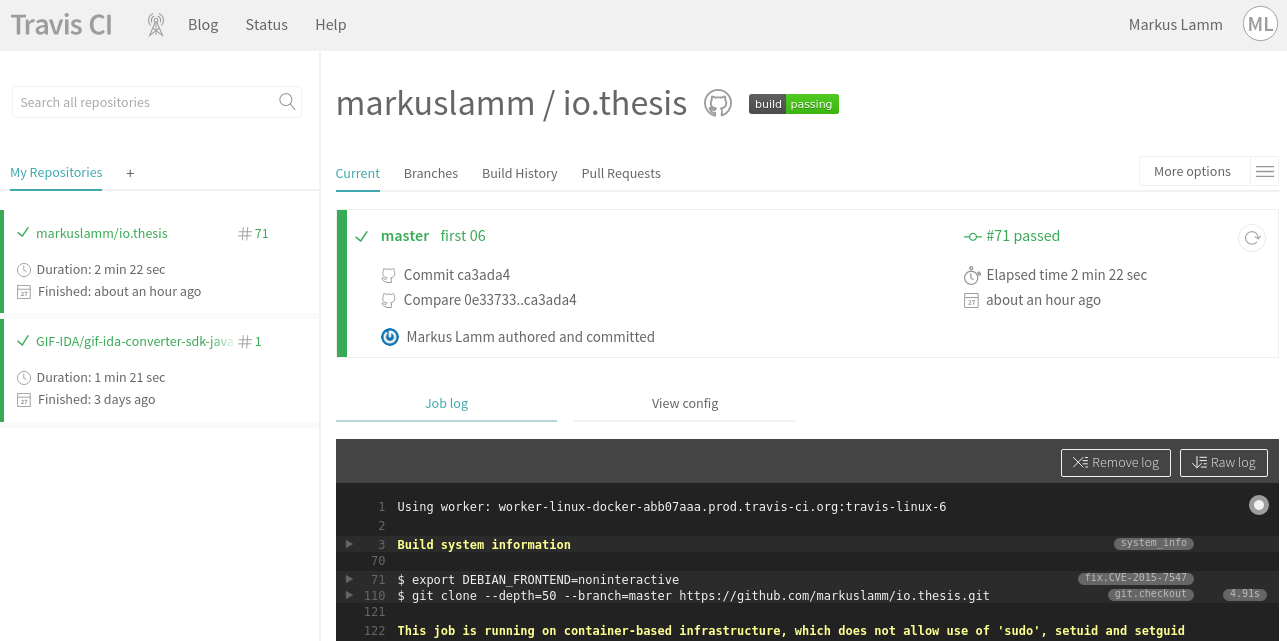
\includegraphics[width=1.0\textwidth]{../images/07-travis.png}
	\caption{Travis CI}
	\label{fig:travis}
\end{figure}

\section{Docker environment}
%The application was developed and is working with the following software components:
%
%* ubuntu 16.04 LTS
%* oracle java 8
%* maven 3.3.3
%* docker 1.11.2
%* docker-compose 1.7.1
local cluster
Short Docker intro, benefits in microservice environments, describe setup for components (docker-compose.yml),
describe modifications made for Apache Flink and Apache Kafka to enable JMX remote access

\begin{figure}[H]
	\centering
	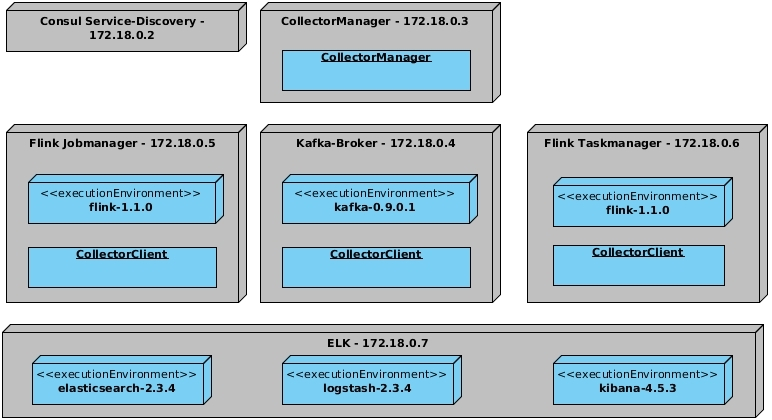
\includegraphics[width=1.0\textwidth]{../uml/deployment-diagram.jpg}
	\caption{Docker Deployment diagram}
	\label{img:deployment-diagram}
\end{figure}

Build images



%\section{Observations}
%
%CollectorDataProcessor: module to analyze the data streams creating derived streams and persist flat
%data -> data transformation, analytics layer
%
%Kibana dashboard, show visualization of CollectorDataProcessor data

\section{Discussion}
%Wurden Sie überrascht? Stimmten Ihre Hypothesen? Sind Sie besser, anders als das andere System?
%Wichtigster Erkenntnisgewinn 1
%Wichtigster Erkenntnisgewinn 2
%Wichtigster Erkenntnisgewinn N
%Anwendbarkeit? Szenario?
\section{Summary}

TODO

%Beschreibung  der Ergebnisse, Diagramme, Darstellen von Zusammenhängen